\documentclass{beamer}
\usetheme{tokitex}

\usepackage{tikz}
\usepackage{graphics}
\usepackage{multirow}
\usepackage{tabto}

\usepackage[english,bahasa]{babel}
\newtranslation[to=bahasa]{Section}{Bagian}
\newtranslation[to=bahasa]{Subsection}{Subbagian}

\usepackage{listings, lstautogobble}
\usepackage{color}

\definecolor{dkgreen}{rgb}{0,0.6,0}
\definecolor{gray}{rgb}{0.5,0.5,0.5}
\definecolor{mauve}{rgb}{0.58,0,0.82}

\lstset{frame=tb,
  language=c++,
  aboveskip=1mm,
  belowskip=1mm,
  showstringspaces=false,
  columns=fullflexible,
  keepspaces=true,
  basicstyle={\small\ttfamily},
  numbers=none,
  numberstyle=\tiny\color{gray},
  keywordstyle=\color{blue},
  commentstyle=\color{dkgreen},
  stringstyle=\color{mauve},
  breaklines=true,
  breakatwhitespace=true,
  autogobble=true
}

\usepackage{caption}
\captionsetup[figure]{labelformat=empty}

\newcommand{\progTerm}[1]{\texttt{#1}}
\newcommand{\foreignTerm}[1]{\textit{#1}}
\newcommand{\newTerm}[1]{\alert{\textbf{#1}}}
\newcommand{\emp}[1]{\alert{#1}}
\newcommand{\statement}[1]{"#1"}


\title{Halo Dunia}
\author{Tim Olimpiade Komputer Indonesia}
\date{}

\newcommand{\compilehelo}{\texttt{g++ -o prog halo.cpp}}

\begin{document}

\begin{frame}
\titlepage
\end{frame}

\begin{frame}
\frametitle{Pendahuluan}
Melalui dokumen ini, kalian akan:
\begin{itemize}
  \item Mengenal program, pemrograman, dan bahasa pemrograman
  \item Memahami bagaimana program dieksekusi
  \item Mengenal kompilator
  \item Mengenal bahasa C++
  \item Melakukan instalasi perangkat lunak yang dibutuhkan untuk pemrograman C++
\end{itemize}
\end{frame}

\section{Perkenalan Pemrograman}
\frame{\sectionpage}

\begin{frame}
\frametitle{Apa itu Program?}
\begin{block}{Program}
  Serangkaian instruksi yang dieksekusi oleh mesin untuk mencapai suatu tujuan tertentu.
\end{block}
\begin{itemize}
  \item Biasanya, program dapat menerima masukan, memprosesnya, dan menghasilkan suatu keluaran.
  \item Contoh: program penerjemah bahasa menerima berkas dalam suatu bahasa sebagai masukan, menerjemahkannya, lalu menghasilkan keluaran berupa hasil terjemahan.
\end{itemize}
\end{frame}

\begin{frame}
\frametitle{Pemrograman dan Bahasa Pemrograman}
\begin{itemize}
  \item Pemrograman adalah aktivitas menulis program.
  \item Program ditulis dengan bahasa pemrograman, sehingga mesin atau komputer dapat mengerti apa yang yang diinstruksikan.
  \item Contoh bahasa pemrograman yang populer adalah C, C++, Pascal, Java, dan Python.
  \item Pada pembelajaran ini, kita akan menggunakan bahasa C++.
\end{itemize}
\end{frame}

\begin{frame}
\frametitle{Bagaimana Komputer Menjalankan Program?}
\begin{itemize}
  \item Pada masa lalu, komputer diprogram dengan bahasa Assembly.
  \item Bahasa Assembly mudah dimengerti oleh mesin. Oleh karena itu, Bahasa Assembly termasuk dalam bahasa pemrograman tingkat rendah (dekat dengan mesin).
  \item Meskipun begitu, membaca dan mengerti alur program Assembly cukup sulit bagi manusia.
\end{itemize}
\end{frame}

\begin{frame}
\frametitle{Bagaimana Komputer Menjalankan Program? (lanj.)}
\begin{itemize}
  \item Pada tahun 1960-an, mulai diciptakan bahasa pemrograman tingkat tinggi.
  \item Bahasa ini lebih mudah dimengerti manusia karena menggunakan frase bahasa sehari-hari, seperti "jika ... maka ..." dan "lakukan ... hingga tercapai ...".
  \item Sayangnya, bahasa pemrograman tingkat tinggi tidak bisa dimengerti secara langsung oleh mesin.
\end{itemize}
\end{frame}

\begin{frame}
\frametitle{Bagaimana Komputer Menjalankan Program? (lanj.)}
\begin{itemize}
  \item Perlu ada penerjemahan bahasa pemrograman tingkat tinggi ke tingkat rendah, sehingga mesin dapat mengerti instruksi yang diberikan.
  \item Penerjemahan ini biasa dilakukan oleh program yang berperan sebagai kompilator, intepreter, atau keduanya. Dalam hal ini kita hanya akan membahas tentang kompilator.
\end{itemize}
\end{frame}

\begin{frame}
\frametitle{Kompilator}
\begin{itemize}
  \item Merupakan program komputer yang dapat menerjemahkan bahasa pemrograman tingkat tinggi ke bahasa mesin.
  \item Hasil terjemahan ini dapat dimengerti oleh mesin, sehingga dapat dieksekusi oleh komputer denga mudah.
  \item Aktivitas menerjemahkan ini disebut dengan kompilasi.
  \item Siklus kerja jika kita menggunakan kompilator adalah: tulis~program $\rightarrow$ kompilasi $\rightarrow$ eksekusi.
\end{itemize}
\end{frame}

\begin{frame}
\frametitle{Mengapa C++?}
\begin{itemize}
  \item Kompilasi berjalan dengan cepat.
  \item Memiliki \foreignTerm{library} berupa \foreignTerm{Standard Template Library} (STL) yang lengkap, sehingga berbagai komponen pemrograman tidak perlu Anda buat ulang.
\end{itemize}
\end{frame}

\section{Petunjuk Mempersiapkan \newline Lingkungan Belajar}
\frame{\sectionpage}

\begin{frame}
\frametitle{Instalasi Dev C++ (Windows)}
\begin{itemize}
  \item Kita akan melakukan instalasi Dev C++, yaitu perangkat lunak gratis untuk memprogram C++.
  \item Seluruh petunjuk instalasi yang akan diberikan ini akan dilakukan pada sistem operasi Windows 7.
  \item Proses instalasi berikut akan menghasilkan dua hal muncul pada komputer kalian, yaitu:
  \begin{itemize}
    \item Kompilator C++ yang bernama g++.
    \item IDE (\textit{Integrated Development Environment}) bawaan dari Dev C++. IDE ini bisa dianggap sebagai sebuah lingkungan tempat kalian memprogram nantinya.
  \end{itemize}
\end{itemize}
\end{frame}

\begin{frame}
\frametitle{Instalasi Dev C++ (Windows)}
\begin{itemize}
  \item Buka \textit{browser} kalian dan kunjungi \href{https://sourceforge.net/projects/orwelldevcpp}{https://sourceforge.net/projects/orwelldevcpp}.
  \item Unduh sesuai dengan arsitektur prosesor komputer kalian, misalnya intel dan Windows 32 bit.
\end{itemize}
\end{frame}

\begin{frame}
\frametitle{Instalasi Dev C++ (Windows) (lanj.)}
\begin{itemize}
  \item Berikut ini adalah tampilan dari https://sourceforge.net/projects/orwelldevcpp
  \item Tekan "Download" untuk mendapatkan Dev C++.
\end{itemize}
\begin{figure}
  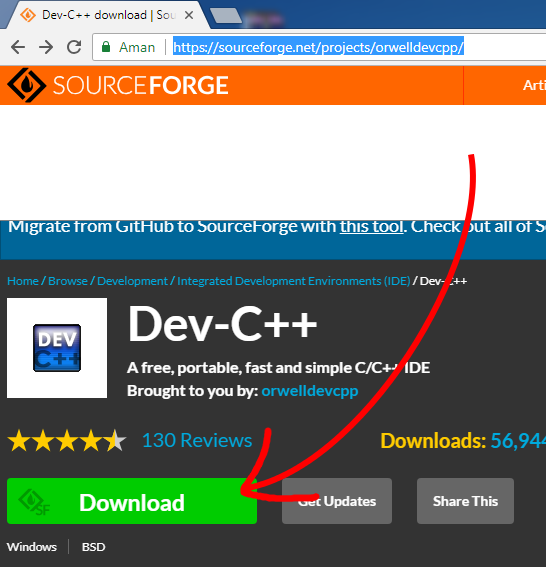
\includegraphics[width=5cm]{asset/devcpp-0.png}
\end{figure}
\end{frame}

\begin{frame}
\frametitle{Instalasi Dev C++ (Windows) (lanj.)}
\begin{itemize}
  \item Setelah selesai mengunduh, jalankan \textit{installer} Dev C++ yang baru saja diunduh.
  \item Akan muncul tampilan sebagai berikut:
  \begin{figure}
    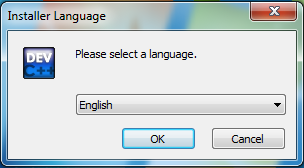
\includegraphics[width=5cm]{asset/devcpp-1.png}
  \end{figure}
\end{itemize}
\end{frame}

\begin{frame}
\frametitle{Instalasi Dev C++ (Windows) (lanj.)}
\begin{itemize}
  \item Baca persetujuan yang ditampilkan.
  \item Setelah Anda menyetujui, tekan "I Agree".
  \begin{figure}
    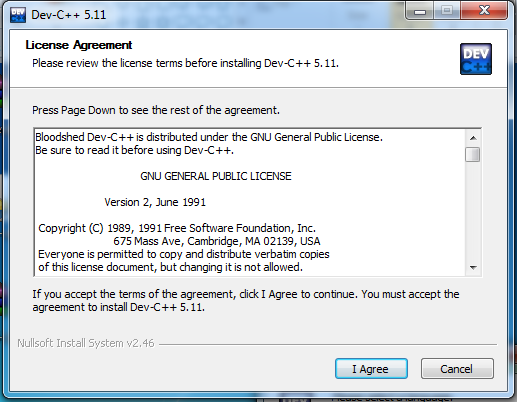
\includegraphics[width=6cm]{asset/devcpp-2.png}
  \end{figure}
\end{itemize}
\end{frame}

\begin{frame}
\frametitle{Instalasi Dev C++ (Windows) (lanj.)}
\begin{itemize}
  \item Selanjutnya, tekan "next" untuk melakukan instalasi.
  \begin{figure}
    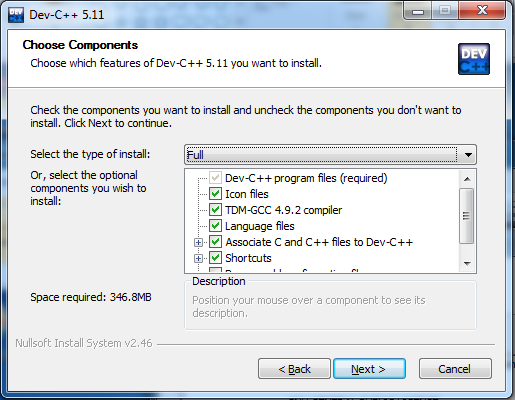
\includegraphics[width=6cm]{asset/devcpp-3.png}
  \end{figure}
\end{itemize}
\end{frame}

\begin{frame}
\frametitle{Instalasi Dev C++ (Windows) (lanj.)}
\begin{itemize}
  \item Atur di mana Anda hendak menyimpan Dev C++.
  \item Ingat di mana lokasinya, lalu tekan "install".
  \begin{figure}
    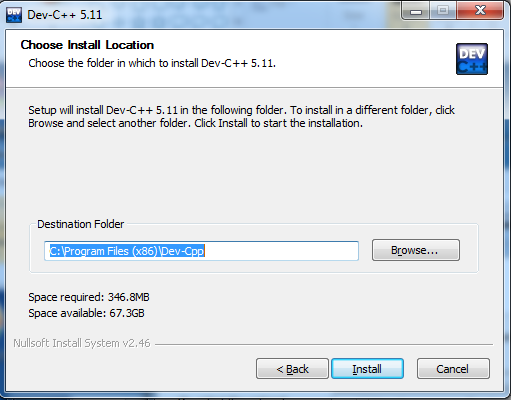
\includegraphics[width=6cm]{asset/devcpp-4.png}
  \end{figure}
\end{itemize}
\end{frame}

\begin{frame}
\frametitle{Instalasi Dev C++ (Windows) (lanj.)}
\begin{itemize}
  \item Tunggu sampai proses instalasi selesai.
  \begin{figure}
    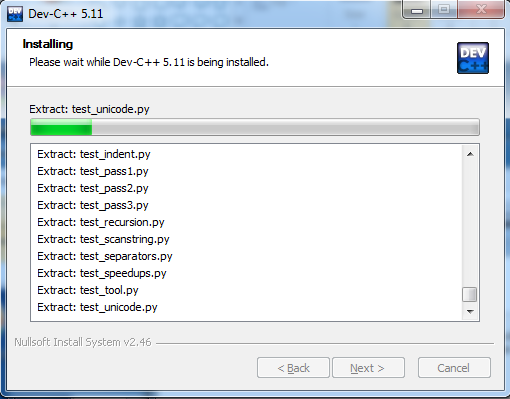
\includegraphics[width=6cm]{asset/devcpp-5.png}
  \end{figure}
\end{itemize}
\end{frame}

\begin{frame}
\frametitle{Instalasi Dev C++ (Windows) (lanj.)}
\begin{itemize}
  \item Jika sudah selesai, pilih \textit{next} dan \textit{finish}.
  \begin{figure}
    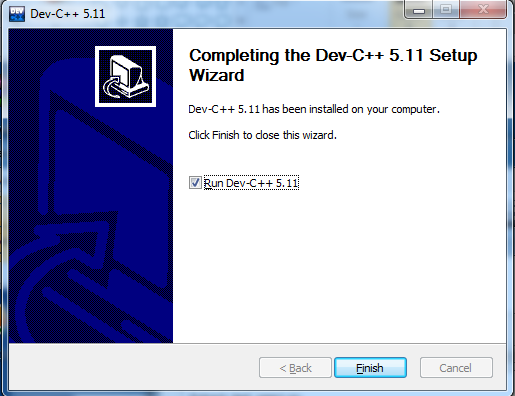
\includegraphics[width=6cm]{asset/devcpp-6.png}
  \end{figure}
\end{itemize}
\end{frame}

\begin{frame}
\frametitle{Instalasi Dev C++ (Windows) (lanj.)}
\begin{itemize}
  \item Jika kalian menjalankan program Dev C++, akan muncul jendela untuk pengaturan.
  \item Setelah selesai mengatur, muncul tampilan berikut:
  \begin{figure}
    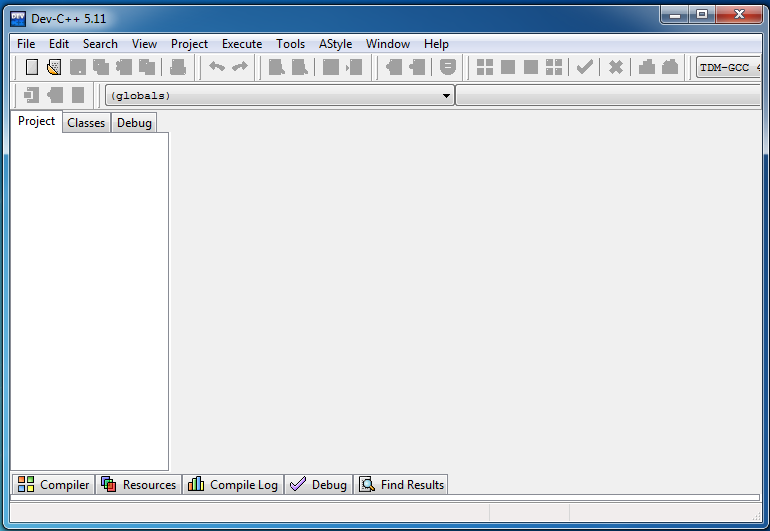
\includegraphics[width=7cm]{asset/devcpp-7.png}
  \end{figure}
\end{itemize}
\end{frame}

\begin{frame}
\frametitle{Lingkungan Pemrograman}
\begin{itemize}
  \item Sejauh ini, memprogram dengan Dev C++ sudah bisa dilakukan.
  \item Untuk membiasakan diri di lingkungan memprogram yang asing, kami memperkenalkan penggunaan \textit{text editor} yang cukup populer, yaitu Notepad++.
  \item Kalian akan menulis kode di Notepad++, lalu melakukan kompilasi dan eksekusi program di \textit{command line}. 
\end{itemize}
\end{frame}

\begin{frame}
\frametitle{Perkenalan Notepad++}
\begin{itemize}
  \item Notepad++ merupakan perangkat lunak pengolah teks gratis yang berjalan di sistem operasi Windows.
  \item Sesuai dengan namanya, kalian bisa menganggap bahwa Notepad++ merupakan versi "plus-plus" dari Notepad, yang mana membuatnya lebih canggih dari Notepad.
  \item Kalian dapat menggunakan Notepad++ untuk berbagai keperluan, seperti menulis program dalam bahasa C, C++, atau Pascal.
\end{itemize}
\end{frame}

\begin{frame}
\frametitle{Instalasi Notepad++ (Windows)}
\begin{itemize}
  \item Buka kembali \textit{browser} kalian, dan kunjungi http://notepad-plus-plus.org/download/v6.7.html
  \begin{figure}
    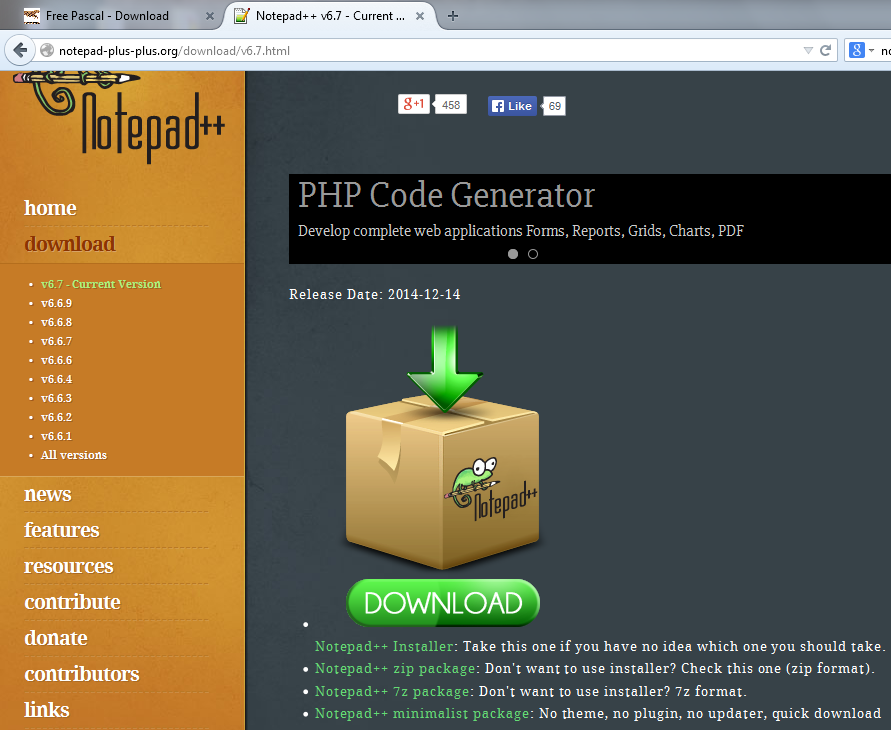
\includegraphics[width=6cm]{asset/npp_1.PNG}
  \end{figure}
  \item Unduh \textit{installer} Notepad++ dengan memilih \textit{Notepad++ Installer} di bagian bawah tombol \textit{download}.
\end{itemize}
\end{frame}

\begin{frame}
\frametitle{Instalasi Notepad++ (Windows) (lanj.)}
\begin{itemize}
  \item Jalankan \textit{installer} Notepad++ yang baru kalian unduh.
  \item Akan muncul tampilan sebagai berikut:
  \begin{figure}
    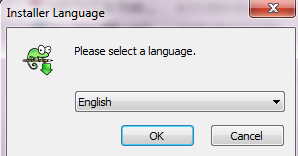
\includegraphics[width=3cm]{asset/npp_3.PNG}
  \end{figure}
  \item Pilih \textit{ok}, lalu \textit{next} sampai muncul tampilan berikut:
  \begin{figure}
    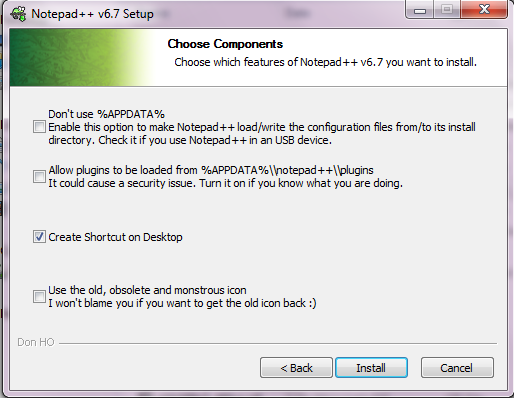
\includegraphics[width=5cm]{asset/npp_7.PNG}
  \end{figure}
\end{itemize}
\end{frame}

\begin{frame}
\frametitle{Instalasi Notepad++ (Windows) (lanj.)}
\begin{itemize}
  \item Pilih \textit{install}, dan tunggu sampai proses instalasi selesai.
  \item Setelah muncul tampilan berikut, pilih \textit{finish}.
  \begin{figure}
    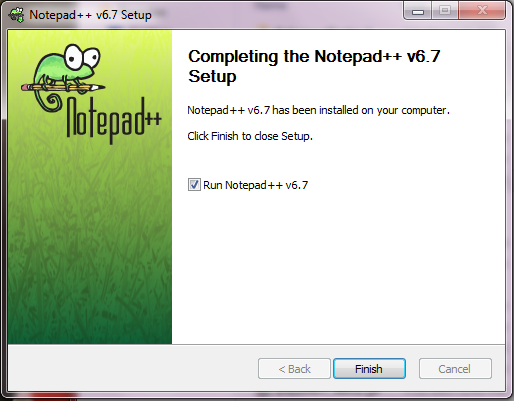
\includegraphics[width=5cm]{asset/npp_9.PNG}
  \end{figure}
\end{itemize}
\end{frame}

\begin{frame}[fragile]
\frametitle{Menulis Program C++ Sederhana}
\begin{itemize}
  \item Ketikkan program berikut pada Notepad++, lalu simpan dengan nama halo.cpp di suatu direktori, misalnya di Documents.
\end{itemize}
\begin{lstlisting}
#include <cstdio>

int main() {
  printf("halo dunia\n");
}
\end{lstlisting}
\end{frame}

\begin{frame}
\frametitle{Kompilasi Program C++}
\begin{itemize}
  \item Buka cmd, yang bisa dilakukan dengan cara menekan tombol winkey+r, lalu isikan "cmd" pada kotak dialog yang muncul, dan tekan enter.
  \begin{figure}
    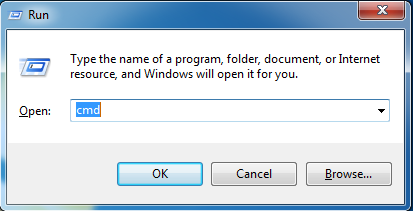
\includegraphics[width=7cm]{asset/run.png}
  \end{figure}
\end{itemize}
\end{frame}

\begin{frame}
\frametitle{Kompilasi Program C++ (lanj.)}
\begin{itemize}
  \item Pergi ke direktori tempat halo.cpp disimpan, gunakan perintah "cd .." untuk mundur ke direktori \textit{parent} dan "cd $<$nama folder$>$" untuk maju ke direktori $<$nama folder$>$.
  \begin{figure}
    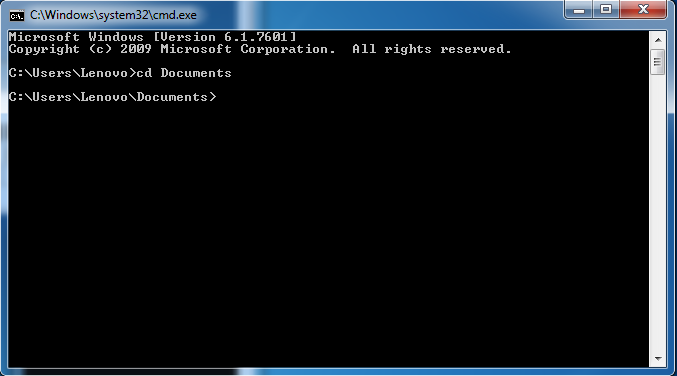
\includegraphics[width=9cm]{asset/cmd-1.png}
  \end{figure}
\end{itemize}
\end{frame}

\begin{frame}
\frametitle{Kompilasi Program C++ (lanj.)}
\begin{itemize}
  \item Ketikkan perintah \compilehelo.
  \item Perhatikan bahwa mungkin akan muncul pesan kesalahan seperti berikut ini:
  \begin{figure}
    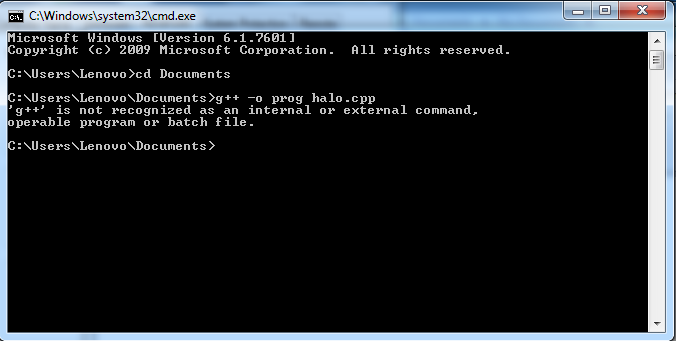
\includegraphics[width=9cm]{asset/cpp-compile-1.png}
  \end{figure}
\end{itemize}
\end{frame}

\begin{frame}[fragile]
\frametitle{Kompilasi Program C++ (lanj.)}
\begin{itemize}
  \item Berikut pesan kesalahan yang diberikan:
\end{itemize}
\begin{quote}
'g++' is not recognized as an internal or external command, operable program or batch file.
\end{quote}
\begin{itemize}
  \item Jika ini terjadi, artinya perlu pengaturan \textit{path} g++ pada \textit{environment variable} terlebih dahulu.
\end{itemize}
\end{frame}

\begin{frame}
\frametitle{Pengaturan \textit{environment variable}}
\begin{itemize}
  \item Klik kanan pada "my computer", lalu pilih \textit{properties}. Akan muncul tampilan sebagai berikut:
  \begin{figure}
    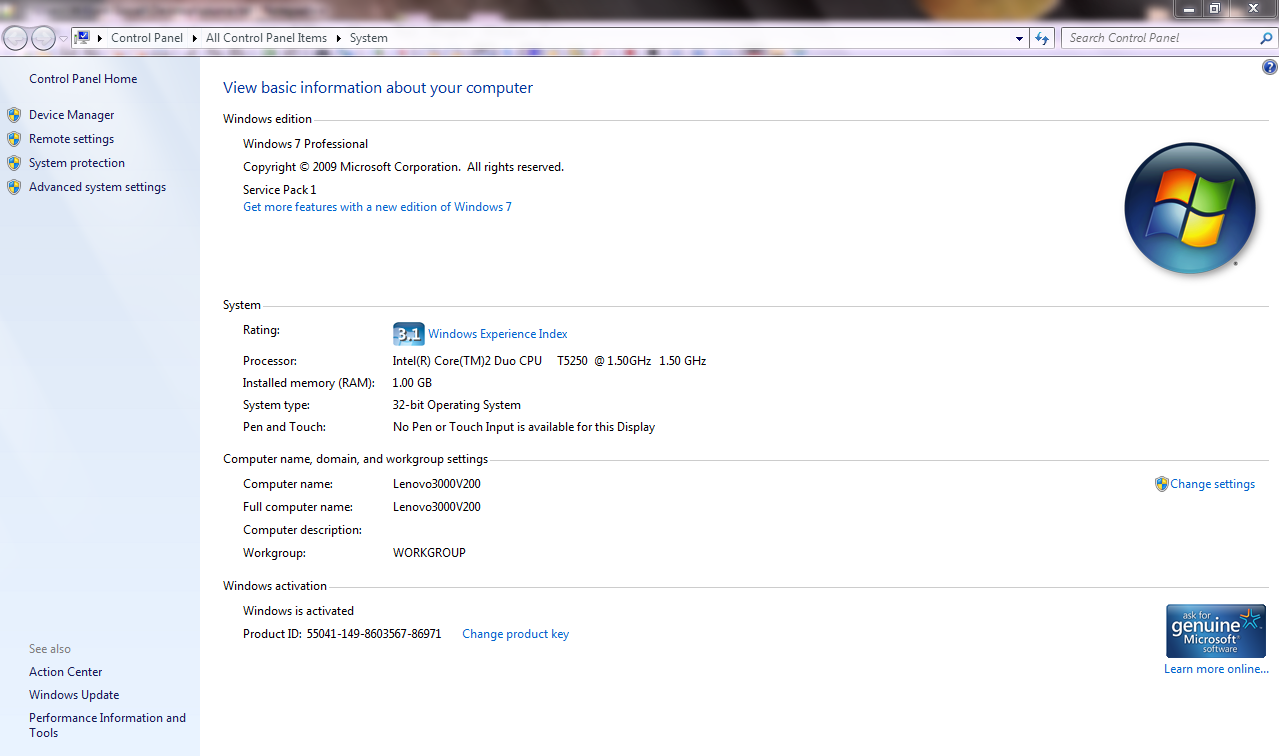
\includegraphics[width=10cm]{asset/path_1.PNG}
  \end{figure}
  \item Pilih \textit{advanced system settings} di bagian kiri.
\end{itemize}
\end{frame}

\begin{frame}
\frametitle{Pengaturan \textit{environment variable} (lanj.)}
\begin{itemize}
  \item Pilih tab \textit{advance}, lalu tekan tombol \textit{environment variable}.
  \begin{figure}
    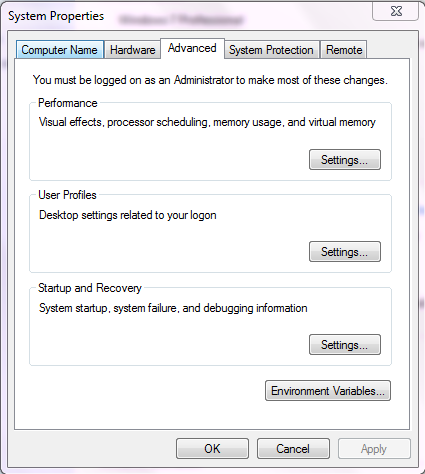
\includegraphics[width=6cm]{asset/path_2.PNG}
  \end{figure}
\end{itemize}
\end{frame}

\begin{frame}
\frametitle{Pengaturan \textit{environment variable} (lanj.)}
\begin{itemize}
  \item Kemudian akan muncul tampilan sebagai berikut:
  \begin{figure}
    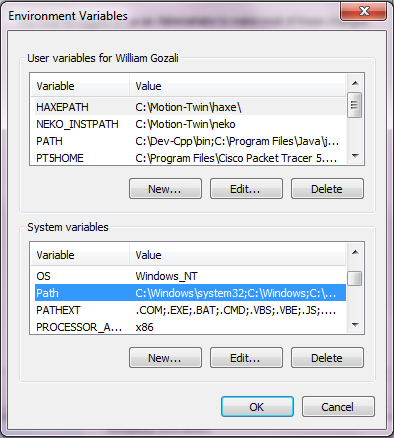
\includegraphics[width=6cm]{asset/path_3.PNG}
  \end{figure}
\end{itemize}
\end{frame}

\begin{frame}
\frametitle{Pengaturan \textit{environment variable} (lanj.)}
\begin{itemize}
  \item Pada bagian \textit{system variables}, pilih \textit{Path} lalu tekan tombol \textit{edit}. Jika kalian tidak bisa menemukannya, maka tekan tombol \textit{new}.
  \item Isikan direktori tempat Dev C++ yang sebelumnya diatur, ditambah dengan "\textbackslash MinGW64\textbackslash bin" pada bagian akhir.
  \begin{figure}
    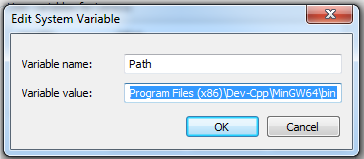
\includegraphics[width=6cm]{asset/cpp-compile-2.png}
  \end{figure}
  \item Tekan \textit{ok} hingga seluruh kotak dialog tertutup.
\end{itemize}
\end{frame}

\begin{frame}
\frametitle{Pengaturan \textit{environment variable} (lanj.)}
\begin{itemize}
  \item Tutup cmd yang telah terbuka, lalu buka kembali.
  \item Pergi ke direktori tempat halo.cpp disimpan dan ketikkan \\ \compilehelo.
  \item Pastikan tidak ada lagi pesan kesalahan yang muncul:
  \begin{figure}
    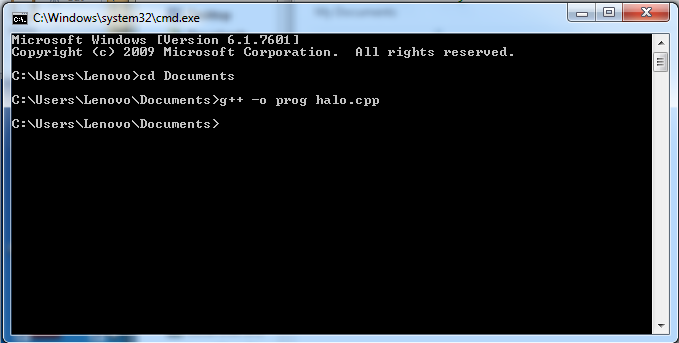
\includegraphics[width=9cm]{asset/cpp-compile-3.png}
  \end{figure}
  \item Selamat! Kompilasi berhasil dilaksanakan!
\end{itemize}
\end{frame}

\begin{frame}
\frametitle{Kompilasi Program C++ (lanj.)}
\begin{itemize}
  \item Ketikkan "prog" pada cmd, yang artinya menjalankan berkas "prog" yang merupakan hasil kompilasi program "helo.cpp".
  \item Pastikan tulisan "halo dunia" tercetak di cmd:
  \begin{figure}
    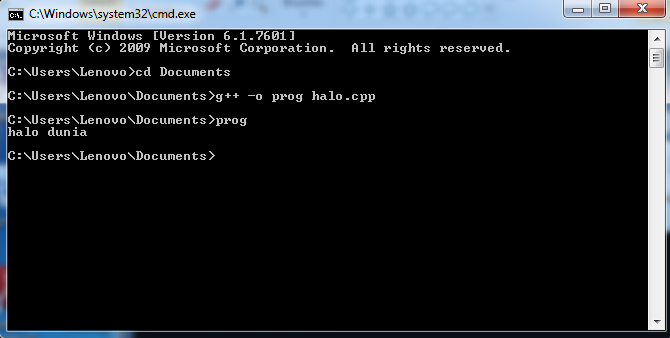
\includegraphics[width=9cm]{asset/cpp-compile-4.png}
  \end{figure}
  \item Selamat! Kalian berhasil menulis dan menjalankan program C++!
\end{itemize}
\end{frame}

\begin{frame}
\frametitle{Penjelasan Cara Kompilasi}
\begin{itemize}
  \item Perintah yang digunakan untuk kompilasi adalah:\\
  \texttt{g++ -o <nama\_berkas> <nama\_program>}
  \item \texttt{<nama\_berkas>} diisi dengan nama berkas hasil kompilasi yang Anda inginkan.
  \item \texttt{<nama\_program>} diisi dengan nama berkas C++ yang hendak Anda kompilasi.
\end{itemize}
\end{frame}

\begin{frame}
\frametitle{Selanjutnya...}
\begin{itemize}
  \item Perkenalan variabel dan tipe data.
  \item Pemrograman C++ sederhana.
\end{itemize}
\end{frame}

\end{document}
